\chapter{Der Gillespie-Algorithmus}
\section{Funktionsweise}
Die Idee hinter dem Gillespie-Algorithmus ist biochemische Systeme anhand von Einzelreaktionen über Zeit stochastisch zu simulieren und so ihre Zusammensetzung zu einem Zeitpunkt t oder nach n Reaktionen herauszufinden, ohne das System selbst beobachten zu müssen.\\
Dabei werden den Reaktionen eigene Wahrscheinlichkeitsmaße $a_{\nu}$ zugeordnet. Diese richten sich nach der Zahl der möglichen Kombinationen vorhandener Ausgangsstoffe $h_{\nu}$ und anderen für die Reaktion wichtigen Parametern, wie beispielsweise der Reaktionsgeschwindigkeit, dem Reaktionsvolumen und der Temperatur, welche alle in die stochastische Ratenkonstante $c_{\nu}$ einfließen (können). Welche Werte hier tatsächlich benötigt werden, hängt von der Anwendung ab. Die Summe aller Wahrscheinlichkeitsmaße $a_{0}$ zu einem Zeitpunkt ergibt ein Maß für die Gesamtreaktivität des Systems. Abhängig von diesem Maß wird der nächste Zeitschritt $\tau$ berechnet, sodass genau eine Reaktion stattfinden kann. Anschließend wird abhängig von $a_{0}$ die Reaktion $\mu$ berechnet, die in $\tau$ stattfinden wird. Abschließend werden die Zähler für Zeit $t$ und Reaktionenzahl $n$ erhöht. Danach beginnt der Algorithmus mit dem nächsten Schritt, indem er die $h_{\nu}$ und $a_{\nu}$ neu berechnet. (Siehe auch \ref{fig:Gillespie-Algorithmus})

\begin{figure}[h]
	\centering
	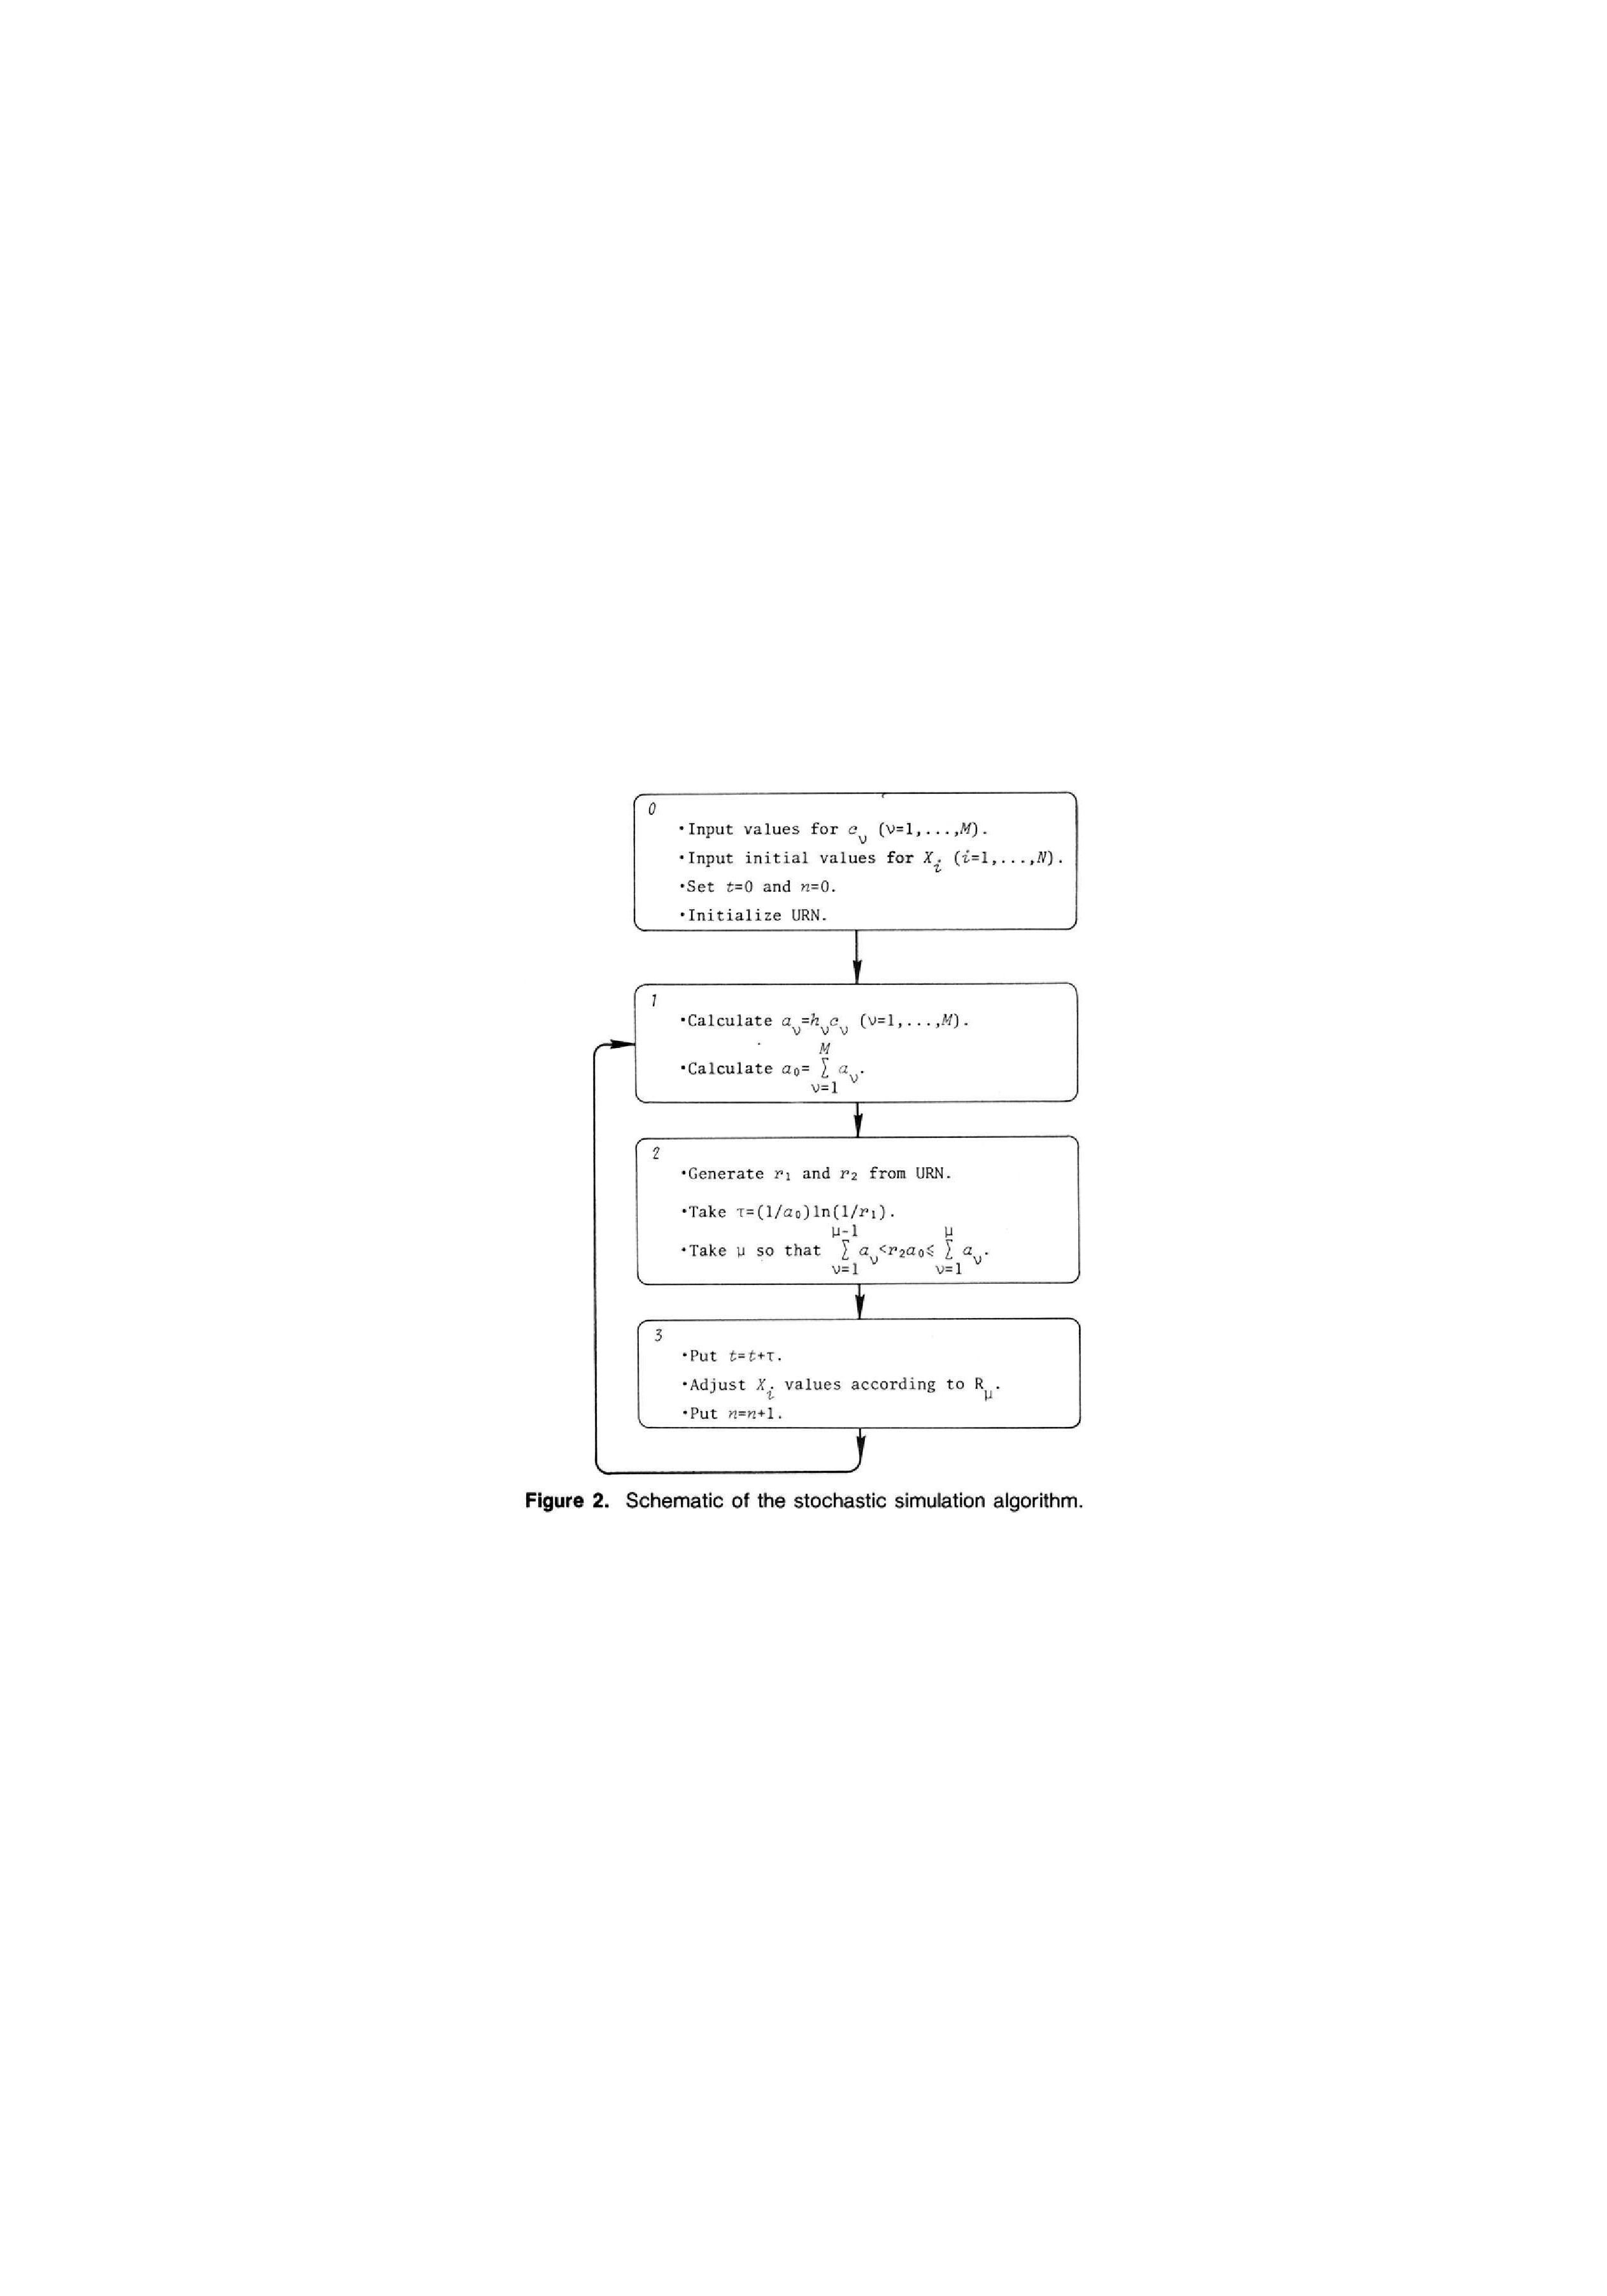
\includegraphics[height=10cm]{Bilder/Gillespie_workflow}
	\caption[justification=raggedright]{Ablauf des Gillespie-Algorithmus\cite{Gillespie1977}\label{fig:Gillespie-Algorithmus}}
\end{figure}


\section{Implementierung}
Die Umsetzung des Algorithmus erfolgte in Programmiersprache Python.\\
Als Input benötigt der Algorithmus jeweils eine Aufstellung der Anfangsquantitäten in Form der stöchiometrischen Matrizen $L$ (alle Spezies, die für eine Reaktion benötigt werden, linke Seite der Reaktion) und $N$ (Gesamtumsatz der Reaktionen), die stochastischen Ratenkonstanten $rateConstants$ für die einzelnen Reaktionen, die Anfangsanzahlen der einzelnen Analyten $startQuantities$ und eine Abbruchbedingung in Form einer maximalen Zeit $time_max$ oder einer maximalen Reaktionenzahl $reaction_limit$. Die Matrix $N$ kann dabei als Differenz aus $R-L$ berechnet werden, wobei $R$ die stöchiomtrische Matrix aller Reaktionsprodukte (rechte Seite der Reaktion) darstellt.
\begin{verbatim}
	class Gillespie():
	def __init__(self, L, N, rConstants, quantities):
\end{verbatim}
Der Gillespie-Algorithmus wurde nach der Beschreibung in dem von Daniel T. Gillespie 1977 veröffentlichten Paper\cite{Gillespie1977} implementiert. Dabei wurden die Zeit- (Liste von \texttt{float}s) und Quantitätsreihen (absolute Anzahlen je Spezies als \texttt{int}) der einzelnen Spezies separat abgespeichert, um diese später gegeneinander plotten zu können.\par

Die generierten Simulationsdaten wurden dann hinsichtlich ihrer Varianz untersucht, um den Zeitpunkt zu berechnen, ab dem das biologische System eingeschwungen ist, also in seinem Gleichgewichtszustand (engl.: steady state) verweilt. In diesem steady state wurde dann das Signal-Rausch-Verhältnis (engl.: signal-to-noise-ratio, kurz SNR) ermittelt. Das SNR gibt das Verhältnis vom Gesamtsignal zum Rauschsignal an und wird berechnet, indem das Gesamtoutputsignal durch das Rauschsignal geteilt wird.\\
Aufgrund der stochastischen Nautur des Gillespie-Algorithmus kann man Aussagen über das Gesamtsystem nur treffen, wenn mehrere Simulationen mit den gleichen Ausgangsbedingungen in die Überlegungen einbezogen wurden, da eine sonst abgelesene Auffälligkeit lediglich dem Zufall geschuldet sein kann. Aus diesem Grund wurde eine Monte-Carlo-Simulation implementiert, welche eine bestimmte Anzahl an Gillespie-Simulationen hintereinander laufen lässt.\par

Um mit dem Algorithmus simulieren zu können muss der Benutzer entweder\newline
\texttt{run\_time\_sec(tmax)} oder \texttt{run\_n\_reactions(nreactions)} in einer Pythonumgebung ausführen. Dabei wird der jeweiligen Methode das Abbruchkriterium für die Simulation übergeben. \texttt{tmax} ist ein \texttt{float}-Zeitwert bei dem der Algorithmus stoppt, wenn er diesen überschreitet und \texttt{nreactions} gibt als \texttt{int}-Wert die maximale Anzahl von Reaktionen an. Beide Methoden speichern schrittweise die Zeit- und Quantitätsdaten der Simulation im Gillespie-Objekt.

\subsection{Ermittlung der stochastischen Ratenkonstanten}
Die stochastischen Ratenkonstanten sind der Dreh- und Angelpunkt. Von ihnen hängt maßgeblich ab, wie sich das simulierte System im Laufe der Zeit verhalten wird.

\subsection{Monte-Carlo-Simulation}
Auf den Gillespie-Algorithmus aufbauend wurde eine Monte-Carlo-Simulation implementiert. Der Standardwert für die Anzahl der nacheinander zu simulierenden Gillespies liegt bei 50. Als Abbruchbedingung soll entweder \texttt{time\_max} oder\newline
\texttt{reaction\_limit} übergeben werden.\newline
\texttt{def monte\_carlo\_gillespie(rateConstants, L, N, startQuantities,\newline
	runs=50, time\_max=None, reaction\_limit=None)}
	
Die Parameter $rateConstants$, $L$, $N$ und $startQuantities$ werden dann für jede Simulation an den Konstruktor der Klasse \texttt{Gillespie} weitergegeben. Rückgabewert der Methode ist eine List mit Gillespie-Objekten.

\subsection{Diagramme}
Um sich die Daten der Simulationen anzeigen zu lassen gibt es ein paar plot-Funktionen. Direkt auf dem Gillespie-Objekt kann man die Funktion \texttt{plot(self, colours=None, outfile="temp\_plot")} ausführen. Dabei kann eine individuell gewählte Färbung für die einzelnen Spezies im System übergeben, sowie ein Speicherort für das Diagramm gewählt werden.\par

Mit der Methode \texttt{multiplot(gillespies, x\_size=None, y\_size=None,\newline
	colours=None, outfile="temp\_multiplot")} können dann mehrere Gillespie-Läufe nebeneinander in einem Bild geplottet werden. Dazu wird intern die Funktion\newline \texttt{pyplot.subplots()} aufgerufen. Der Nutzer muss hier eine Liste von mehreren Gillespie-Objekten\newline \texttt{gillespies} übergeben und kann bei Bedarf mit \texttt{x\_size} und \texttt{y\_size} die Maße des Diagramm-Arrays festlegen oder mit \texttt{outfile} einen eigenen Ausgabepfad wählen.\par

Um die Streuung in der Monte-Carlo-Simulation zu veranschaulichen wurde die Methode \texttt{analyte\_plot(gillespies, x\_size=None, y\_size=None, colours=None, outfile="temp\_analyte\_plot")} implementiert. Mit dieser werden die einzelnen Molekülspezies der Simulationsläufe jeweils zusammen geplottet, sodass gut zu sehen ist wie sich die einzelnen Spezies über alle Läufe entwickelt haben. Es wird wieder eine Liste von Gillespie-Läufen \texttt{gillespies} verlangt, alle anderen Parameter sind optional.\par

\texttt{make\_output\_signal(list\_gillespies, output\_species\_names)} ist dazu gedacht das Gesamtoutputsignal aus allen Sonden-bindenden Spezies zu berechnen. Dazu werden, zusätzlich zur schon bekannten Liste der Gillespie-Objekte, die Speziesnamen, welche das Outputsignal ausmachen, als Liste von Strings übergeben. Rückgabewert ist eine Liste, die nur die nach den einzelnen Läufen geteilten Quantitäten für das Outputsignal enthält.

\subsection{Statistische Analyse}
Um die Rauschleistung des simulierten biologischen Systems analysieren zu könnenimplementiert, die die verschiedenen Gillespie-Läufe in Fenstern festzulegender Größe (Standard sind 100 Werte) nach ihrer Varianz gleitend mit der Schrittweite $step_size$ untersucht. Wenn die Änderung der Varianz von Fenster zu Fenster einen festzulegenden Schwellwert (Standard sind 0.05, also 5\%) unterschreitet, wird der Zeitpunkt bei dem dies passiert als cut-off gespeichert. Anschließend wird aus allen cut-offs das Maximum $t_trimming$ gezogen, um sicher zu gehen, dass das System in allen Läufen eingeschwungen ist.
\begin{verbatim}
	def get_trimming_time(list_gillespies, window_length=10, step_width=None,
	vct=0.05)
\end{verbatim}

Bei der weiteren Berechnung werden für die SNR nur noch diejenigen Datenpunkte mit einbezogen, deren Zeitwerte größer als t\_trimming sind.
Weiterhin können der Variationskoeffizient, die Standardabweichungen und die Mittelwerte der Molekülquantitäten berechnet werden.
